%% CS6215 course project report.
%% ACM Primary Article Template (acmart, sigconf).
%% Limit: 6-10 pages main text (incl. figures, tables, appendices, AI Use Statement) + <= 1 page references.
%%
%% Build:  python -m nesy evaluate                      (results/summary/*.csv)
%%         python scripts/make_report_assets.py         (report/figures/*.pdf, report/tables/*.tex)
%%         cd report && latexmk -pdf main_revised2.tex
%% Every number in the tables, and the numbers in the text written as macros (\VFourDet, ...), comes from
%% report/tables/*.tex, so re-running the commands above after labelling updates the report.
%% Label-based numbers (\NumLabelled, \VFourPrec, ...) come from labels/*.csv via the same commands.
\documentclass[sigconf]{acmart}
\settopmatter{printacmref=false, printfolios=true}
\setcopyright{none}
\acmConference[CS6215 Advanced Topics in Program Analysis]{Symbolic Program Analysis vs Neurosymbolic Program Analysis}{}{National University of Singapore}
\acmYear{}\acmDOI{}\acmISBN{}
% Suppress wall-clock PDF metadata; scholarly reference years remain intact.
\ifdefined\pdfinfoomitdate\pdfinfoomitdate=1\fi
\ifdefined\pdftrailerid\pdftrailerid{}\fi
\renewcommand\footnotetextcopyrightpermission[1]{}

\usepackage{booktabs}
\usepackage{multirow}
\usepackage{tikz}
\usetikzlibrary{positioning,arrows.meta,fit,calc}
\usepackage{xcolor}
\usepackage{listings}
\lstdefinestyle{code}{basicstyle=\ttfamily\scriptsize, columns=fullflexible, keepspaces=true, frame=tb,
  framerule=0.4pt, aboveskip=4pt, belowskip=2pt, xleftmargin=2pt, numbers=none, breaklines=true,
  commentstyle=\color{black!55}, keywordstyle=\bfseries, showstringspaces=false}
\lstset{style=code}
\emergencystretch=1.2em
\newcommand{\tool}{\textsc{NESY-Taint}}
\newcommand{\cwe}[1]{CWE-#1}
% Generated by scripts/make_report_assets.py -- do not edit by hand.
\newcommand{\BOneAlarms}{496}
\newcommand{\BOneAlarmsFixed}{505}
\newcommand{\BOneConf}{0}
\newcommand{\BOneConfRate}{0\%}
\newcommand{\BOneDet}{1}
\newcommand{\BOneDiff}{0}
\newcommand{\BOneFDR}{0.86}
\newcommand{\BOneFOne}{0.11}
\newcommand{\BOneLab}{90}
\newcommand{\BOneLabIMP}{63}
\newcommand{\BOneLabSPEC}{0}
\newcommand{\BOneLabTP}{5}
\newcommand{\BOnePrec}{0.01}
\newcommand{\BOneRate}{25\%}
\newcommand{\BOneTPRate}{25\%}
\newcommand{\BOneTPRep}{1}
\newcommand{\BTwoAlarms}{1,511}
\newcommand{\BTwoAlarmsFixed}{1,525}
\newcommand{\BTwoConf}{4}
\newcommand{\BTwoConfRate}{100\%}
\newcommand{\BTwoDet}{4}
\newcommand{\BTwoDiff}{2}
\newcommand{\BTwoFDR}{0.44}
\newcommand{\BTwoFOne}{0.59}
\newcommand{\BTwoLab}{227}
\newcommand{\BTwoLabIMP}{184}
\newcommand{\BTwoLabSPEC}{0}
\newcommand{\BTwoLabTP}{11}
\newcommand{\BTwoPrec}{0.51}
\newcommand{\BTwoRate}{100\%}
\newcommand{\BTwoTPRate}{100\%}
\newcommand{\BTwoTPRep}{4}
\newcommand{\CrashRuns}{8}
\newcommand{\FallbackDrivers}{6}
\newcommand{\IrisAlarms}{1,865}
\newcommand{\IrisAlarmsFixed}{1,925}
\newcommand{\IrisConf}{2}
\newcommand{\IrisConfRate}{50\%}
\newcommand{\IrisDet}{3}
\newcommand{\IrisDiff}{1}
\newcommand{\IrisFDR}{0.68}
\newcommand{\IrisFOne}{0.20}
\newcommand{\IrisLab}{379}
\newcommand{\IrisLabIMP}{212}
\newcommand{\IrisLabSPEC}{113}
\newcommand{\IrisLabTP}{10}
\newcommand{\IrisPrec}{0.01}
\newcommand{\IrisRate}{58\%}
\newcommand{\IrisTPRate}{50\%}
\newcommand{\IrisTPRep}{2}
\newcommand{\NovalRuns}{48}
\newcommand{\NumFlows}{6,523}
\newcommand{\NumLLMRuns}{192}
\newcommand{\NumLabClaude}{436}
\newcommand{\NumLabDRV}{47}
\newcommand{\NumLabFP}{423}
\newcommand{\NumLabIMP}{252}
\newcommand{\NumLabSAN}{7}
\newcommand{\NumLabSPEC}{117}
\newcommand{\NumLabTP}{13}
\newcommand{\NumLabelled}{436}
\newcommand{\NumRuns}{208}
\newcommand{\PctLabDRV}{11\%}
\newcommand{\PctLabIMP}{60\%}
\newcommand{\PctLabSAN}{2\%}
\newcommand{\PctLabSPEC}{28\%}
\newcommand{\TotalCalls}{12,845}
\newcommand{\VFourAlarms}{289}
\newcommand{\VFourAlarmsFixed}{563}
\newcommand{\VFourConf}{3}
\newcommand{\VFourConfRate}{58\%}
\newcommand{\VFourDet}{4}
\newcommand{\VFourDiff}{3}
\newcommand{\VFourFDR}{0.52}
\newcommand{\VFourFOne}{0.54}
\newcommand{\VFourLab}{223}
\newcommand{\VFourLabIMP}{122}
\newcommand{\VFourLabSPEC}{57}
\newcommand{\VFourLabTP}{13}
\newcommand{\VFourPrec}{0.33}
\newcommand{\VFourRate}{83\%}
\newcommand{\VFourTPRate}{75\%}
\newcommand{\VFourTPRep}{4}
\newcommand{\VOneAlarms}{1,918}
\newcommand{\VOneAlarmsFixed}{2,041}
\newcommand{\VOneConf}{3}
\newcommand{\VOneConfRate}{67\%}
\newcommand{\VOneDet}{4}
\newcommand{\VOneDiff}{2}
\newcommand{\VOneFDR}{0.62}
\newcommand{\VOneFOne}{0.37}
\newcommand{\VOneLab}{403}
\newcommand{\VOneLabIMP}{227}
\newcommand{\VOneLabSPEC}{117}
\newcommand{\VOneLabTP}{11}
\newcommand{\VOnePrec}{0.06}
\newcommand{\VOneRate}{83\%}
\newcommand{\VOneTPRate}{67\%}
\newcommand{\VOneTPRep}{3}
\newcommand{\VThreeAlarms}{269}
\newcommand{\VThreeAlarmsFixed}{44}
\newcommand{\VThreeConf}{1}
\newcommand{\VThreeConfRate}{25\%}
\newcommand{\VThreeDet}{2}
\newcommand{\VThreeDiff}{2}
\newcommand{\VThreeFDR}{0.84}
\newcommand{\VThreeFOne}{0.16}
\newcommand{\VThreeLab}{149}
\newcommand{\VThreeLabIMP}{64}
\newcommand{\VThreeLabSPEC}{55}
\newcommand{\VThreeLabTP}{10}
\newcommand{\VThreePrec}{0.05}
\newcommand{\VThreeRate}{42\%}
\newcommand{\VThreeTPRate}{42\%}
\newcommand{\VThreeTPRep}{2}
\newcommand{\VTwoAlarms}{295}
\newcommand{\VTwoAlarmsFixed}{114}
\newcommand{\VTwoConf}{2}
\newcommand{\VTwoConfRate}{42\%}
\newcommand{\VTwoDet}{4}
\newcommand{\VTwoDiff}{4}
\newcommand{\VTwoFDR}{0.59}
\newcommand{\VTwoFOne}{0.32}
\newcommand{\VTwoLab}{186}
\newcommand{\VTwoLabIMP}{90}
\newcommand{\VTwoLabSPEC}{60}
\newcommand{\VTwoLabTP}{11}
\newcommand{\VTwoPrec}{0.10}
\newcommand{\VTwoRate}{67\%}
\newcommand{\VTwoTPRate}{58\%}
\newcommand{\VTwoTPRep}{3}


% acmart's hyperxmp also supplies dates and a clock-seeded instance identifier.
\makeatletter
\AtBeginDocument{%
  \@ifpackageloaded{hyperxmp}{%
    \let\hyxmp@today@xmp\@empty
    \let\hyxmp@today@pdf\@empty
    \let\@pdfcreationdate\@empty
    \let\@pdfmoddate\@empty
    \let\@pdfdatetime\@empty
    \let\@pdfmetadatetime\@empty
    \let\hyxmp@InstanceID\@empty
    \def\hyxmp@def@InstanceID{}%
  }{}%
}
\makeatother

\begin{document}

\title[Comparing Symbolic and Neuro-Symbolic Taint Analysis]{Comparing Symbolic and Neuro-Symbolic Taint Analysis\\ for Java Vulnerabilities}
\author{Jia Yu Lim}
\affiliation{\institution{National University of Singapore}\city{Singapore}\country{Singapore}}
\email{jiayu.lim@u.nus.edu}
\renewcommand{\shortauthors}{Jia Yu Lim}


\begin{abstract}
In this project, we compared symbolic and neuro-symbolic static taint analysis on four Java CVEs covering path traversal, code injection and command injection. Then, we evaluated a configured symbolic baseline, a curated symbolic specification, an IRIS-style pipeline, and staged combinations of large language model (LLM) specification inference, driver generation and alarm triage, all using Tai-e as the propagation engine. We analysed buggy and fixed versions, repeated each LLM configuration three times, and measured detection, alarm counts, cost and failure causes. Runtime witnesses confirmed each vulnerability independently of patch-location metrics and LLM flow labels.

We found out that inferred specifications improved coverage, generated drivers sharply reduced alarms but sometimes missed required entry points, and triage removed harmless flows but also rejected a real vulnerability. Symbolic validation prevented the specification-induced crashes seen in our ablations, but cannot tell whether a sink is dangerous or a route is feasible. The curated symbolic baseline reached all four witness-validated sinks, which showed how much specification quality matters.

These findings motivate \tool{}, which added driver checks, array-element sinks and a rule that stops triage from dismissing recognised sinks as harmless. It reported patch-relevant flows to the witness-validated sinks for all four CVEs in at least one run per subject, with an \VFourRate{} per-run patch-method detection rate and \VFourAlarms{} alarms per run summed across subjects, compared with \BTwoAlarms{} for the curated baseline and \IrisAlarms{} for the IRIS-style pipeline. Because these rules were developed on the same four subjects, we do not declare general superiority or novelty based on the results.
\end{abstract}


\begin{CCSXML}
<ccs2012>
<concept><concept_id>10011007.10011074.10011099.10011102.10011103</concept_id>
<concept_desc>Software and its engineering~Software testing and debugging</concept_desc><concept_significance>300</concept_significance></concept>
<concept><concept_id>10011007.10010940.10010992.10010998.10011000</concept_id>
<concept_desc>Software and its engineering~Automated static analysis</concept_desc><concept_significance>500</concept_significance></concept>
<concept><concept_id>10002978.10003022.10003023</concept_id>
<concept_desc>Security and privacy~Software security engineering</concept_desc><concept_significance>300</concept_significance></concept>
</ccs2012>
\end{CCSXML}
\ccsdesc[500]{Software and its engineering~Automated static analysis}
\ccsdesc[300]{Security and privacy~Software security engineering}
\keywords{taint analysis, neuro-symbolic program analysis, large language models, specification inference, Tai-e}

\maketitle
\fancyhead[LE,RO]{\footnotesize CS6215 Advanced Topics in Program Analysis, National University of Singapore}
\noindent\textbf{Student ID:} A0358309W \quad \textbf{GitHub Repository:} \url{https://github.com/Pyrexiaa/CS6215_Neurosymbolic_Program_Analysis}

% =====================================================================================================

\section{Introduction}
Path traversal, command injection and code injection occur when attacker-controlled input reaches a sensitive operation without an effective check. Static taint analysis identifies potential vulnerabilities by tracking data from untrusted \emph{sources} to sensitive \emph{sinks}. Its usefulness depends on more than the propagation algorithm as the analyzer must start from relevant entry points, recognise the right sources and sinks, and distinguish dangerous flows from harmless ones.

These requirements are hard to meet for libraries and framework-based applications. A library may lack a suitable main method, a plugin may depend on framework callbacks, and a generic specification can miss a project-specific sink. Even with suitable inputs, a conservative analysis can join unrelated program paths and report many alarms. Large language models (LLMs) can supply the missing API knowledge and judge the resulting alarms. IRIS~\cite{li2025iris}, for example, uses LLMs to infer taint specifications and to triage CodeQL alarms in context. However, a plausible model answer is not necessarily a valid analysis input or a correct security judgement.

This study asks where LLM assistance helps static taint analysis, where it fails, and which symbolic checks address the observed failures. All configurations use Tai-e~\cite{tan2023taie} for propagation, so they differ only in their analysis inputs and alarm handling. We compare two symbolic baselines (Tai-e's configured specification and a curated version with additional project-specific taint rules), an IRIS-style pipeline built on Tai-e, and four configurations that add specification inference, driver generation, triage and targeted symbolic rules one step at a time.

We evaluate on four CVEs from CWE-Bench-Java~\cite{li2025iris}, each with a buggy and a fixed version, and measure detection in three ways: the overlap with the patched methods, flow labels from an LLM judge, and runtime witnesses that reproduce each vulnerability and check if the fix blocks it. These measures can disagree because an alarm can touch a patched method while tracking the wrong input, and a model can reject a flow that reaches an exploitable sink.

There is no LLM stage that improves every outcome. Inferred specifications broaden coverage, generated drivers cut alarms from \VOneAlarms{} to \VTwoAlarms{} but sometimes miss a required entry point, and triage removes harmless flows but also one real vulnerability. The curated symbolic specification remains strong, reaching all four witness-validated sinks with \BTwoAlarms{} alarms. From these failures we built \tool{} (v4), which extends the initial pipeline (v3) with driver checks, array-element sinks and a rule that stops triage from dismissing recognised sinks. It reaches the same four sinks in at least one run per subject with \VFourAlarms{} alarms, about a fifth as many. Because these rules were developed on the same subjects explicitly, this result motivates but does not establish a general improvement.

Therefore, our contributions are:

\begin{enumerate}
    \item \textbf{Controlled comparison.}
    We compare symbolic and neuro-symbolic taint analysis
    on one engine, examine each LLM stage, and ablate
    the specification and triage validators.

    \item \textbf{Failure analysis.}
    We analyse successes and failures using three forms
    of evidence: patch-method overlap, LLM-judged labels
    and runtime witnesses.

    \item \textbf{Strengthened approach and artifact.}
    We present \tool{} and a reproducible artifact containing
    its rules, prompts, run records, provisional labels
    and scripts.
\end{enumerate}

\section{Related Work}
\label{sec:related}
\textbf{Symbolic analysis and entry modelling.} Tai-e~\cite{tan2023taie} provides the Java pointer and taint analyses used in this study. FlowDroid~\cite{arzt2014flowdroid} models the Android lifecycle, and JackEE~\cite{antoniadis2020jackee} models enterprise Java frameworks; both show that modelling entry points is part of the analysis itself. We study whether an LLM can generate a useful analysis driver and which checks its output needs.

\textbf{Specification inference and alarm triage.} SuSi~\cite{rasthofer2014susi} uses machine learning to classify Android APIs as sources and sinks, and Seldon~\cite{chibotaru2019seldon} infers taint specifications from large code corpora. IRIS~\cite{li2025iris} is the closest work to ours. We reuse its benchmark and patch-location metrics, but build a separate pipeline on Tai-e that also generates drivers and validates specifications. LLift~\cite{li2024llift} and Wen et al.~\cite{wen2024llm4sa} also use LLMs to inspect static-analysis warnings. Our staged comparison shows when such inspection reduces alarms and when it loses a real vulnerability.

\textbf{Validating LLM output.} LLMDFA~\cite{wang2024llmdfa}, LLMSAN~\cite{wang2024llmsan}, NESA~\cite{wang2024nesa} and RepoAudit~\cite{guo2025repoaudit} combine LLM reasoning with program-based evidence or checks. KNighter~\cite{yang2025knighter} uses LLMs to synthesise static checkers, and LLM-based fuzz-driver generation~\cite{zhang2024fuzzdriver} repairs generated code using compiler feedback. For this project, our checks are narrower as they validate driver compilation and calls, specification structure and cited evidence, but do not prove reachability, sanitisation or exploitability.

\section{Preliminaries}
\label{sec:prelim}
\subsection{Taint Analysis and Example}
A taint specification lists \emph{sources} of untrusted data, \emph{sinks} where that data can cause harm, \emph{transfers} that carry taint through library calls, and \emph{sanitizers} that remove it. The analyzer reports each source-to-sink flow as an \emph{alarm}. We study path traversal (\cwe{22}), code injection (\cwe{94}) and OS command injection (\cwe{78}).

Listing~\ref{lst:ztzip} shows \mbox{CVE-2018-1002201}, a Zip Slip vulnerability in zt-zip. The attacker controls the name of an archive entry (line~1). If the name contains \texttt{../}, the file created at line~3 can lie outside the output directory, and extraction then writes outside it. Detection therefore needs a source for the entry name and a sink on the second argument of the \texttt{File(File, String)} constructor, the child path. Tai-e's configured specification lacks this source and marks only the first argument, the parent directory, as a sink. Finding the right method is not enough: the specification must also mark the right argument.

\begin{lstlisting}[language=Java, numbers=left, numberstyle=\tiny\color{black!55}, numbersep=4pt, xleftmargin=9pt, caption={Zip Slip in zt-zip (abridged). The archive entry name (line~1) controls the child path; the output directory is a trusted input.}, label=lst:ztzip]
String name = mapper.map(zipEntry.getName());
if (name != null) {
    File file = new File(outputDir, name);
    // Write the archive entry to file.
}
\end{lstlisting}

\subsection{Tai-e and the Shared Configuration}
Tai-e (v0.5.4) builds a call graph and points-to sets from an entry method. Its taint analysis creates taint objects at source calls, propagates them through assignments, fields, arrays, calls and returns, and reports a flow when a sink's configured position may point to a taint object. The analysis is flow-insensitive, so a reported flow is a possible relation, not proof of an attack.

A specification entry names a method and a position: the receiver, the result, a zero-based argument, or the elements of an array argument. An array and its elements are different targets, which matters for command injection, where commands are often string arrays. Tai-e also outputs a taint flow graph (TFG) of potential taint propagation through program and library nodes; we use it as triage evidence and to match alarms to patched methods. In call-site mode, rules match the method named at the call site, so rules on library interfaces fire without an analysed implementation. When library bodies are skipped, taint crosses a library call only through a transfer rule.

All configurations use the JDK~8 library, call-site mode and \texttt{1-call} context sensitivity, which analyses a method separately for each calling site. Experiments on small test programs led to two changes from Tai-e's commonly used configuration: \texttt{1-call} reduces unrelated string flows that merge through a shared string builder, and removing three string-copy transfer rules stops taint from spreading through internal JDK buffers. For perfecto-plugin, whole-program analysis exceeded the 6\,GB heap, so every configuration skips library bodies for this subject and adds generated transfer rules for string-builder chaining.

For libraries without a suitable main method, Tai-e needs a driver which is a synthetic main method that calls entry points with tainted arguments. The symbolic baselines use a template driver that calls up to 300 ranked public methods, taints every string, stream and file parameter, and shares one receiver object per class. This broad model can taint trusted inputs, such as the output directory in Listing~\ref{lst:ztzip}. B1 uses Tai-e's specification for the relevant CWE with the changes above; B2 adds a curated specification (Section~\ref{sec:setup}).


\section{Approach}
\label{sec:approach}
\begin{figure*}[t]
\centering
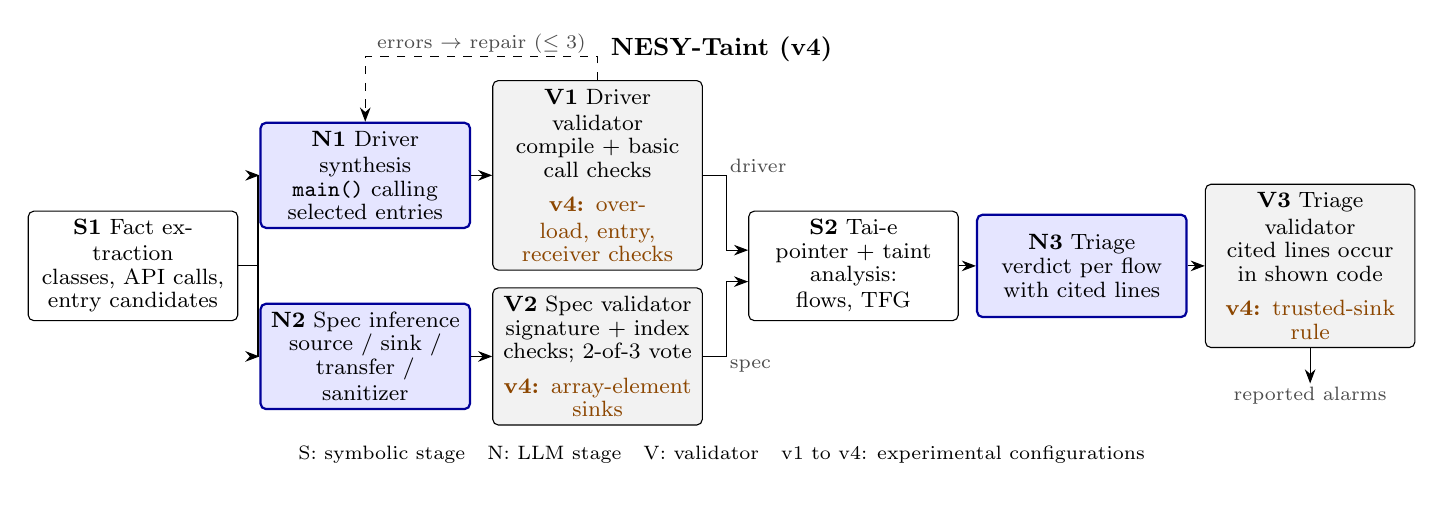
\begin{tikzpicture}[>={Stealth[length=1.8mm]}, font=\footnotesize,
  box/.style={draw, rounded corners=2pt, align=center, minimum height=13mm, text width=24.5mm, inner sep=3pt, fill=white},
  llm/.style={box, fill=blue!10, draw=blue!60!black, thick},
  val/.style={box, fill=gray!10},
  lab/.style={font=\scriptsize, text=black!70, align=center, inner sep=1pt}]
  \node[font=\small\bfseries] at (7.475,2.75) {\tool{} (v4)};
  \node[box] (s1) at (0,0) {\textbf{S1} Fact extraction\\[-1pt] classes, API calls,\\[-1pt] entry candidates};
  \node[llm] (n1) at (2.95, 1.15) {\textbf{N1} Driver synthesis\\[-1pt] \texttt{main()} calling\\[-1pt] selected entries};
  \node[val] (v1) at (5.9, 1.15) {\textbf{V1} Driver validator\\[-1pt] compile + basic\\[-1pt] call checks\\[3pt] {\color{orange!55!black}\textbf{v4:} overload, entry,\\[-1pt] receiver checks}};
  \node[llm] (n2) at (2.95,-1.15) {\textbf{N2} Spec inference\\[-1pt] source / sink /\\[-1pt] transfer / sanitizer};
  \node[val] (v2) at (5.9,-1.15) {\textbf{V2} Spec validator\\[-1pt] signature + index\\[-1pt] checks; 2-of-3 vote\\[3pt] {\color{orange!55!black}\textbf{v4:} array-element\\[-1pt] sinks}};
  \node[box] (s2) at (9.15,0) {\textbf{S2} Tai-e\\[-1pt] pointer + taint\\[-1pt] analysis: flows, TFG};
  \node[llm] (n3) at (12.05,0) {\textbf{N3} Triage\\[-1pt] verdict per flow\\[-1pt] with cited lines};
  \node[val] (v3) at (14.95,0) {\textbf{V3} Triage validator\\[-1pt] cited lines occur\\[-1pt] in shown code\\[3pt] {\color{orange!55!black}\textbf{v4:} trusted-sink\\[-1pt] rule}};
  \draw[->] (s1.east) -- ++(0.25,0) |- (n1.west);
  \draw[->] (s1.east) -- ++(0.25,0) |- (n2.west);
  \draw[->] (n1) -- (v1);
  \draw[->] (n2) -- (v2);
  \draw[->] (v1.east) -- ++(0.3,0) node[lab, above right] {driver} |- ([yshift=2mm]s2.west);
  \draw[->] (v2.east) -- ++(0.3,0) node[lab, below right] {spec} |- ([yshift=-2mm]s2.west);
  \draw[->] (s2) -- (n3);
  \draw[->] (n3) -- (v3);
  \draw[->, dashed] (v1.north) -- ++(0,0.3) -| node[lab, pos=0.25, above] {errors $\rightarrow$ repair ($\le 3$)} (n1.north);
  \draw[->] (v3.south) -- ++(0,-0.45) node[lab, below] {reported alarms};
  \node[font=\scriptsize, align=center] at (7.475,-2.55) {S: symbolic stage\quad N: LLM stage\quad V: validator\quad v1 to v4: experimental configurations\\[2pt]};
\end{tikzpicture}
\caption{\tool{} in its final configuration, v4. The LLM writes the driver (N1), infers specifications (N2) and triages alarms (N3); validators V1 to V3 check these outputs, and Tai-e performs all propagation. Each validator box marks its v4 additions: overload, declared-entry and receiver checks in V1, array-element sinks in V2, and the trusted-sink rule in V3.}
\Description{The complete pipeline is configuration v4. Capital V1, V2 and V3 identify validators, while lowercase v1 to v4 identify experimental configurations. Fact extraction feeds driver synthesis and specification inference, whose outputs are validated before Tai-e analysis. Tai-e flows pass through LLM triage and the triage validator. Labelled v4 additions appear inside the corresponding validator boxes: overload, entry and receiver checks in V1; array-element sinks in V2; and the trusted-sink rule in V3. Driver errors trigger up to three repair rounds, with a template fallback for persistent compilation or basic-call failures.}
\label{fig:pipeline}
\end{figure*}

\tool{} uses an LLM at three points where the symbolic baseline struggles: entry-point modelling (N1), specification inference (N2) and alarm triage (N3). We label the three LLM stages N1 to N3 and their corresponding
symbolic validators V1 to V3. Lowercase v1 to v4 denote the
experimental configurations compared in this study. Figure~\ref{fig:pipeline} shows the final design (v4). The initial design lacks the three groups of checks and rules described below, which we derived from v3's failures on the evaluated subjects (Section~\ref{sec:rq3}). A symbolic validator checks each LLM output. Persistent compilation or basic-call failures trigger a template fallback. Invalid specification entries are dropped and unsupported alarm removals are rejected. These checks catch structural errors and selected inconsistencies, without proving security correctness.

\subsection{Fact Extraction (S1)}
A class-file parser reads the application, its dependency jars and the JDK~8 library. It extracts the application's methods and line ranges, its calls to external APIs, and a ranked list of entry candidates such as public methods, constructors and framework callbacks, excluding names of common Object methods such as \texttt{equals}. N2 receives one source line from each of up to two call sites per API.

\subsection{Analysis Drivers (N1 and V1)}
To avoid tainting trusted inputs, N1 asks the LLM for a driver that calls attacker-reachable entries and taints only attacker-controlled inputs. The prompt gives the CWE, a README excerpt, the top 60 entry candidates and a small API for creating tainted values. The LLM also lists the entries it intends to call.

V1 compiles the driver for Java~8 with annotation processing disabled and checks that its bytecode calls both application code and the taint API. Errors and failed checks go back to the LLM for up to three repair rounds, after which persistent compilation or basic-call failures trigger the template fallback.

For drivers that compile but do not do what was intended, v4 adds three checks. Bytecode checks flag a call that resolves to an inherited library overload although the application declares a method with the same name and arity, and an entry that the driver lists but never calls. A source-level receiver check flags a driver that sets up one object but calls the entry on another object of the same class. These checks guide repair without proving aliasing or entry coverage; a driver that still fails the entry check after the last repair is kept with a warning.

\subsection{Specification Inference (N2 and V2)}
N2 fills in missing library-specific specifications by labelling each external API as a source, sink, transfer, sanitizer or none. Each prompt holds 25 APIs with their signatures, valid index positions, libraries and call sites. Boilerplate APIs and APIs already configured as sources, transfers or sanitizers are left out, while configured sinks stay visible so that N2 can add a missing argument, such as the child path in Listing~\ref{lst:ztzip}.

V2 checks that inferred rules refer to known APIs and use positions and types supported by Tai-e. Invalid rules are discarded. N2 produces three samples, and a rule is retained only if at least two samples propose it. Each sample contributes at most one vote per rule. These checks establish structural validity and agreement, but not security correctness.

Tai-e tracks array objects and their contents separately. When an accepted sink rule refers to an array argument, v4 also adds a rule for its elements. This allows the sink to detect tainted values stored inside the array, such as an attacker-controlled string in a command array.

\subsection{Alarm Triage (N3 and V3)}
N3 reviews up to 200 flows per run. For each flow, it sees the shortest available TFG route as numbered code snippets with context from up to six application methods. If no complete route exists, it sees the endpoints and the methods reachable from the source or leading to the sink. It answers \texttt{vulnerable}, \texttt{not\_vulnerable} or \texttt{uncertain}, with a reason and the lines it relies on.

Inspired by LLMSAN~\cite{wang2024llmsan}, V3 removes a flow only when a \texttt{not\_vulnerable} verdict cites lines that were actually shown; other verdicts keep the flow. The check confirms that the evidence exists, not that the reasoning is correct.

The v4 trusted-sink rule covers sinks in Tai-e's specification for the CWE and sinks labelled by all three N2 samples. N3 may not remove a flow to such a sink by calling the sink harmless, but can still reject it because of its source, a sanitizer or an infeasible route. Simply put, the rule checks the method not the argument.

% =====================================================================================================


\section{Evaluation}
\label{sec:eval}
\subsection{Research Questions}
\noindent\textbf{RQ1 (Effectiveness).} How do the configurations compare in CVE detection and alarm volume?\par
\noindent\textbf{RQ2 (Contribution).} What does each LLM stage and validator contribute?\par
\noindent\textbf{RQ3 (Failures).} Why do configurations miss CVEs or report false alarms?\par
\noindent\textbf{RQ4 (Practical feasibility).} How do the configurations compare in resource use and stability, and how do resource limits constrain the study?

\subsection{Subjects and Configurations}
\label{sec:setup}
\begin{table}[t]
\caption{Buggy subjects. LoC: non-blank Java lines; Jars: dependency jars; APIs: distinct external APIs called; Fix: methods changed by the patch; Tai-e: B1 analysis time.}
\label{tab:subjects}
\small\setlength{\tabcolsep}{3.2pt}
\begin{tabular}{@{}llrrrrr@{}}
\toprule
Subject & CVE (CWE) & LoC & Jars & APIs & Fix & Tai-e (s) \\
\midrule
zt-zip & 2018-1002201 (Path trav.) & 8,520 & 5 & 196 & 3 & 10.2 \\
spark & 2016-9177 (Path trav.) & 10,486 & 35 & 325 & 7 & 44.5 \\
cron-utils & 2021-41269 (Code inj.) & 7,877 & 32 & 214 & 2 & 9.1 \\
perfecto & 2020-2261 (OS cmd inj.) & 756 & 222 & 106 & 9 & 1.9 \\
\bottomrule
\end{tabular}

\end{table}

\textbf{Subjects.} We selected four CVEs in Maven-buildable projects from CWE-Bench-Java~\cite{li2025iris}, covering three CWE classes and different analysis needs (Table~\ref{tab:subjects}) which included the archive extraction in zt-zip, static-file serving in spark, Bean Validation message evaluation in cron-utils, and shell commands built from job settings in perfecto-plugin. Each has a buggy and a fixed version. We use the benchmark's original buggy revisions and prepare buildable fixed versions with two adjustments. For cron-utils, we apply the two upstream security changes to the buggy revision, retaining its Java~8 build configuration because the upstream fixed revision requires Java~16. For perfecto-plugin, we use the commit immediately following the benchmark-listed fix. It retains the security changes and updates the build and dependency configuration so that the project compiles in our setup.

\begin{table}[t]
\caption{Configurations. All share the Tai-e settings of Section~\ref{sec:prelim}. v1 adds specification inference, v2 driver synthesis, v3 triage and v4 the three groups of checks and rules; the last rows ablate v3's validators.}
\label{tab:configs}
\small\setlength{\tabcolsep}{3pt}
\begin{tabular}{@{}llll@{}}
\toprule
Config & Driver & Specification & Triage \\
\midrule
B1 & template & Tai-e base & none \\
B2 & template & base + curated & none \\
IRIS-style & template & base + N2/V2 & N3/V3 \\
\midrule
v1 & template & base + N2/V2 & none \\
v2 & N1/V1 & base + N2/V2 & none \\
v3 & N1/V1 & base + N2/V2 & N3/V3 \\
v4 & N1/V1 + checks & + array rule & + trusted sinks \\
\midrule
v3 w/o V2 & \multicolumn{3}{l}{v3 without the specification validator} \\
v3 w/o V3 & \multicolumn{3}{l}{v3 without the triage validator} \\
v3 w/o V2+V3 & \multicolumn{3}{l}{both off (V1 must stay on)} \\
\bottomrule
\end{tabular}
\end{table}

\textbf{Configurations.} Table~\ref{tab:configs} lists all configurations. B2's curated specification was written from N2's candidate API lists and buggy source, without consulting advisories or fixes. Earlier B1 results had been seen so B2 is an optimistic curated baseline. IRIS-style is v3 with the template driver instead of N1, which isolates the effect of the driver. The ablations reuse v3's LLM answers with V2, V3 or both disabled. Disabling V2 can change the specification and hence the flows that triage sees. Compilation stays on because Tai-e needs a compiled driver, and the other V1 checks are not ablated.

\textbf{Setup.} All LLM stages use \texttt{qwen3.6:35b} through NUS's SoCLaaS API. N1 and N3 use temperature~0; N2 uses three samples at temperatures 0, 0.7 and 0.7. We repeat each LLM configuration three times, yielding \NumRuns{} records including the deterministic baselines. Tai-e runs on a MacBook Pro with JDK~17 and a 6\,GB heap. The artifact provides the prompts, settings and cached responses needed to reproduce the reported results.

\subsection{Detection Measures}
\label{sec:measures}
\textbf{Automatic metrics.} Before triage, every configuration drops flows with JDK-internal endpoints or driver sinks and merges the rest into source-to-sink flow keys, treating all driver source sites as one and same-line endpoints as one. A flow is \emph{GT-relevant} (relevant to the ground-truth patch) when its source, its sink or a method on its TFG route matches a patched method by package, class and name. The route methods must be reachable from the source and reach the sink, and overloads and line ranges are ignored. Following IRIS, a run detects a CVE if it reports any GT-relevant flow. Per run, precision $P$ is the fraction of reported flows that are GT-relevant; recall $R$ is 1 for detection and 0 otherwise. $\mathrm{FDR}=1-P$ and $F_1=2PR/(P+R)$, with $F_1=0$ for empty runs or $P+R=0$. We average over runs, then subjects while the FDR excludes empty runs. These metrics measure overlap with patched methods, not exploitability, and are not comparable with IRIS's published scores because of the difference between path extraction and aggregation.

\textbf{LLM-judged labels.} To look beyond patch overlap, we labelled a sample of flows. From a frozen sampling frame of 6,582 flow keys, fixed-seed draws took up to 10 GT-relevant and 10 other flows per subject, version and main configuration, taking small strata whole. The overlapping draws give \NumLabelled{} distinct flows, including every cron-utils and perfecto-plugin flow. An LLM judge~\cite{zheng2023judging}, Claude Opus 5.5, labelled each flow from its source, sink, TFG snippets and any N3 verdict. A true-positive (TP) label requires attacker control, a dangerous sink argument, a feasible route and no effective neutralisation. A false-positive (FP) label records which condition fails. Flows sharing a source or sink site were judged together, and the labels were not human-verified (Section~\ref{sec:limits}).

Because the draws overlap, a flow's inclusion probability depends on the draws it was eligible for. If flow $i$ was eligible for draws $D_i$, where draw $d$ samples $n_d$ of $N_d$ flows, then $\pi_i=1-\prod_{d\in D_i}(1-n_d/N_d)$. For a run reporting flows $A$ and the labelled sample $S$, the Horvitz-Thompson estimate of precision is
\[
 \widehat P_{\mathrm{label}}=\frac{1}{|A|}\sum_{i\in S\cap A}\frac{\mathbf{1}[\mathrm{label}_i=\mathrm{TP}]}{\pi_i}.
\]
It corrects for unequal inclusion probabilities but treats the labels as correct. Empty runs have no precision, a nonempty run with no sampled flow contributes zero, and no run has an unlabelled sampled flow or a flow outside the frame. We average over non-empty runs, then subjects, without confidence intervals. The labels also define confirmed detection (a GT-relevant flow judged TP) and TP reported (any reported flow judged TP even outside the patched methods). A subject has a \emph{buggy/fixed differential} when a configuration detects its CVE and reports fewer GT-relevant alarms per run on the fixed version.

\textbf{Runtime witnesses.} To check the four CVEs without flow labels or LLM calls, we wrote one runtime witness per CVE: a harmless proof of concept that exercises the relevant API or handler with attacker-controlled input on the built buggy and fixed versions. Each security effect is reproduced on the buggy version and blocked on the fixed version: an archive entry escapes the extraction directory (zt-zip), a request path resolves to a class outside the static root (spark), the injected expression \texttt{\$\{7*7\}} evaluates to \texttt{49} in a validation message (cron-utils), and an injected job parameter runs a command on the Jenkins controller (perfecto-plugin). A detection is witness-confirmed when a reported GT-relevant flow matches the subject-specific sink family demonstrated by the witness. This is a stricter measure than patch overlap but it does not execute every reported flow.

\subsection{Effectiveness (RQ1)}
\begin{table}[t]
\caption{Buggy-version results on the 4 subjects. B1 and B2 run once; LLM configurations run three
times to measure variation across runs. Det.: CVEs flagged in any run; Rate: percentage of runs reporting a
GT-relevant flow, averaged across subjects; FDR and F1: automatic patch-method metrics. Conf.: subjects with a GT-relevant flow judged TP; TP: subjects with any reported flow judged TP; Prec.: estimated precision, averaged over non-empty runs, then subjects. The labels are not human-verified. Alarms: reported flows per run, summed over subjects.}
\label{tab:headline}
\small\setlength{\tabcolsep}{3.4pt}
\begin{tabular}{@{}lrrrrrrrr@{}}
\toprule
 & \multicolumn{4}{c}{IRIS metrics} & \multicolumn{3}{c}{LLM-judged sample} & \\
\cmidrule(lr){2-5}\cmidrule(lr){6-8}
Config & Det. & Rate & FDR & F1 & Conf. & TP & Prec. & Alarms \\
\midrule
B1 & 1/4 & 25\% & 0.86 & 0.11 & 0/4 & 1/4 & 0.01 & 496 \\
B2 & 4/4 & 100\% & 0.44 & 0.59 & 4/4 & 4/4 & 0.51 & 1,511 \\
IRIS-style & 3/4 & 58\% & 0.68 & 0.20 & 2/4 & 2/4 & 0.01 & 1,865 \\
v1 & 4/4 & 83\% & 0.62 & 0.37 & 3/4 & 3/4 & 0.06 & 1,918 \\
v2 & 4/4 & 67\% & 0.59 & 0.32 & 2/4 & 3/4 & 0.10 & 295 \\
v3 & 2/4 & 42\% & 0.84 & 0.16 & 1/4 & 2/4 & 0.05 & 269 \\
v4 & 4/4 & 83\% & 0.52 & 0.54 & 3/4 & 4/4 & 0.33 & 289 \\
\bottomrule
\end{tabular}

\end{table}

\begin{figure}[t]
\centering
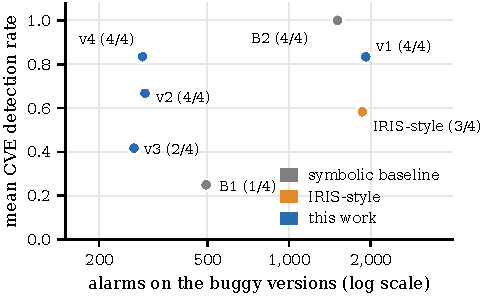
\includegraphics[width=\columnwidth]{figures/detection_vs_alarms.pdf}
\caption{Detection rate versus alarm volume on buggy versions. Labels give the CVEs flagged in any run.}
\Description{Scatter plot of mean detection rate against the number of alarms on a log scale for each configuration. v4 is in the upper left with 4 of 4 CVEs and about 300 alarms. B2 and v1 detect 4 of 4 with 1,500 to 2,000 alarms. IRIS-style 3 of 4 with about 1,900. B1 1 of 4 with about 500.}
\label{fig:scatter}
\end{figure}

Table~\ref{tab:headline} and Figure~\ref{fig:scatter} show the trade-off between coverage and alarms. B1 flags only zt-zip, through driver-modelling false positives (Conf.\ \BOneConf{}/4). Its specification lacks the Bean Validation and array-element sinks, and its five sampled spark TP flows lie outside the patched methods. Inferred specifications (v1) flag all four CVEs with \VOneAlarms{} alarms, and adding triage (IRIS-style) leaves \IrisDet{} CVEs and \IrisAlarms{} alarms. LLM drivers (v2) cut alarms to \VTwoAlarms{}, though v2's perfecto-plugin detection comes from an unrelated sink (RQ2). Triage drops v3 to \VThreeDet{} CVEs while v4 restores all \VFourDet{} with \VFourAlarms{} alarms and the best automatic F1 among LLM configurations (\VFourFOne{}). B2 has the best F1 overall (\BTwoFOne{}) and flags every CVE, but reports \BTwoAlarms{} alarms.

Estimated label precision is \VFourPrec{} for v4, \IrisPrec{} for IRIS-style, \VOnePrec{} for v1 and \BTwoPrec{} for B2, but the two small subjects inflate these averages. On zt-zip and spark, precision stays below 0.2 for every configuration. The estimates rest on few TPs (\VFourLabTP{} of \VFourLab{} judged flows for v4, \BTwoLabTP{} of \BTwoLab{} for B2). GT-relevant TPs confirm v4's detection on \VFourConf{}/4 subjects, against \IrisConf{}/4 for IRIS-style and \BTwoConf{}/4 for B2.

\begin{table}[tb]
\caption{Buggy-version detection by patch-method overlap, LLM judgement and runtime witness. Witness confirmation matches a reported GT-relevant flow to the subject-specific sink family demonstrated by the witness and uses no flow labels.}
\label{tab:witness}
\centering\small\setlength{\tabcolsep}{4pt}
\begin{tabular}{@{}lccc@{}}
\toprule
Config & Patch-method Det. & LLM-judged Conf. & Witness-confirmed \\
\midrule
B1 & 1/4 & 0/4 & 0/4 \\
B2 & 4/4 & 4/4 & 4/4 \\
IRIS-style & 3/4 & 2/4 & 2/4 \\
v1 & 4/4 & 3/4 & 3/4 \\
v2 & 4/4 & 2/4 & 3/4 \\
v3 & 2/4 & 1/4 & 2/4 \\
v4 & 4/4 & 3/4 & 4/4 \\
\bottomrule
\end{tabular}
\end{table}

Table~\ref{tab:witness} compares the three detection measures. B1's detection is not witness-confirmed because its zt-zip alarm reaches the trusted directory argument. The witnesses agree with the judge for B1, B2, v1 and IRIS-style and add one CVE for v2, v3 and v4, showing that spark's resource-read sink, which the judge rejected, is exploitable. Only B2 and v4 are witness-confirmed on all four CVEs.

\begin{table}[t]
\caption{Per-subject detection rate on buggy (B) and fixed (F) versions. B~$>$~F is preferable, but drivers and specifications are inferred separately for each version, which confounds the contrast.}
\label{tab:persubject}
\small\setlength{\tabcolsep}{3.4pt}
\begin{tabular}{@{}lrrrrrrrr@{}}
\toprule
Config & \multicolumn{2}{c}{zt-zip} & \multicolumn{2}{c}{spark} & \multicolumn{2}{c}{cron-utils} & \multicolumn{2}{c}{perfecto} \\
\cmidrule(lr){2-3}\cmidrule(lr){4-5}\cmidrule(lr){6-7}\cmidrule(lr){8-9}
 & B & F & B & F & B & F & B & F \\
\midrule
B1 & 1 & 1 & 0 & 0 & 0 & 0 & 0 & 0 \\
B2 & 1 & 1 & 1 & 1 & 1 & 0 & 1 & 0 \\
IRIS-style & 1 & 1 & 1 & 1 & 0 & 0 & 0.33 & 1 \\
v1 & 1 & 1 & 1 & 1 & 0.67 & 0 & 0.67 & 1 \\
v2 & 1 & 1 & 0.67 & 0 & 0.67 & 0 & 0.33 & 0 \\
v3 & 1 & 0.33 & 0.67 & 0 & 0 & 0 & 0 & 0 \\
v4 & 1 & 0.33 & 0.67 & 0.33 & 0.67 & 0 & 1 & 1 \\
\bottomrule
\end{tabular}

\end{table}

\begin{figure*}[t]
\centering
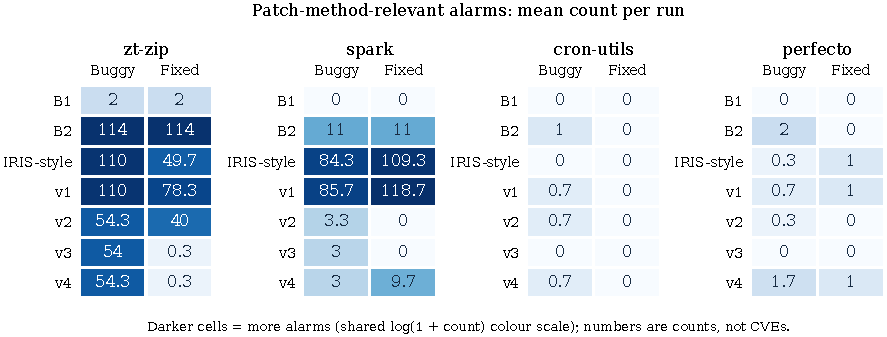
\includegraphics[width=\textwidth]{figures/differential.pdf}
\caption{Mean GT-relevant alarms per run on buggy and fixed versions. Shading uses a shared $\log(1+\mathrm{count})$ scale. Counts are flows, not CVEs or confirmed exploits.}
\Description{Four tables with coloured cells, one per subject. Rows are configurations; columns are buggy and fixed versions. Each cell displays the exact mean count to one decimal where needed, with darker blue for larger counts on a common logarithmic colour scale. Zero is explicitly printed.}
\label{fig:differential}
\end{figure*}

\textbf{Buggy/fixed comparison.} A fixed version should yield fewer GT-relevant alarms than its buggy version (Table~\ref{tab:persubject}, Figure~\ref{fig:differential}). Template-driver configurations flag spark and zt-zip equally often on both versions because the template taints all public-method arguments, including trusted output directories, and so creates alarms at patched methods unrelated to the CVE. LLM drivers remove most fixed-version alarms: the differential holds on \VTwoDiff{}/4 subjects for v2 and \VFourDiff{}/4 for v4, against \BTwoDiff{}/4 for B2 and \IrisDiff{}/4 for IRIS-style. The remaining fixed-version flows include perfecto-plugin's legitimate Jenkins build step and a v4 spark run that fell back to the template.

\begin{table}[tb]
\caption{GT-relevant alarms per run before triage, when each buggy v4 run's driver and specification are reused on the fixed version (mean of three runs).}
\label{tab:paired}
\centering\small
\begin{tabular}{@{}lrr@{}}
\toprule
Subject & Buggy & Fixed \\
\midrule
zt-zip & 54.3 & 54.3 \\
spark & 3.3 & 3.3 \\
cron-utils & 0.7 & 0.0 \\
perfecto-plugin & 2.0 & 0.7 \\
\bottomrule
\end{tabular}

\end{table}

Because drivers and specifications are inferred separately for each version, these differences cannot be attributed to the patch alone. To hold analysis inputs fixed, we reused the driver and specification of each of the 12 buggy v4 runs on the fixed version. All driver calls still resolved and no LLM call was needed as the dependencies were identical except for perfecto-plugin. With these frozen inputs, zt-zip and spark report the same GT-relevant counts on both versions, while cron-utils and perfecto-plugin drop (Table~\ref{tab:paired}). Under these frozen inputs, the fixes do not reduce Tai-e's GT-relevant alarm counts for zt-zip or spark. On fixed zt-zip, independently inferred inputs yield 40 GT-relevant alarms per run before triage and 0.3 after triage, compared with 54.3 under the frozen buggy inputs. The triage removals cite sanitisation and these counts show that both input generation and triage affect the version contrast.

To address RQ1, we designed \tool{} (v4) which matches B2's witness-confirmed coverage with a fifth of the alarms, but has a lower patch-method detection rate (\VFourRate{} versus 100\%).

\subsection{Contribution of Each Stage (RQ2)}
\begin{table}[t]
\caption{Stage effects, LLM usage and stability. Spec/Rej.: N2 labels accepted/rejected per run. Rem./Rem.GT: triage removals per run, all and GT-relevant, summed over the 8 subject versions. V3: removals vetoed by the validator or the trusted-sink rule, on the same basis. Calls: total over 24 runs. Jacc.: mean pairwise Jaccard similarity of alarm sets across the 3 runs. B1 and B2 make no LLM calls.}
\label{tab:cost}
\small\setlength{\tabcolsep}{3.0pt}
\begin{tabular}{@{}lrrrrrrr@{}}
\toprule
Config & Spec & Rej. & Rem. & Rem.GT & V3 & Calls & Jacc. \\
\midrule
IRIS-style & 20.2 & 3.4 & 170 & 40 & 4 & 2,980 & 0.56 \\
v1 & 20.2 & 3.4 & 0 & 0 & 0 & 558 & 0.67 \\
v2 & 20.2 & 3.4 & 0 & 0 & 0 & 604 & 0.63 \\
v3 & 20.2 & 3.4 & 97 & 41 & 1 & 1,689 & 0.52 \\
v4 & 20.2 & 3.4 & 81 & 40 & 27 & 1,947 & 0.41 \\
\bottomrule
\end{tabular}

\end{table}

\textbf{Specification (v1 vs.\ B1).} N2 adds about 20 accepted labels per run (Table~\ref{tab:cost}), supplying the missing sources and sinks and raising detection from 1/4 to 4/4 CVEs. V2 rejects 3.4 labels per run and among the 82 rejections, the largest groups refer to the receiver of a static method (23), a primitive value (25: 17 source or sink arguments and 8 transfer targets) or a nonexistent argument (16).

\textbf{Driver (v2 vs.\ v1).} Driver synthesis gives the largest alarm reduction (\VOneAlarms{} to \VTwoAlarms{} on buggy versions, \VOneAlarmsFixed{} to \VTwoAlarmsFixed{} on fixed), with a differential on all four subjects, but it also changes which entries are called and which inputs count as attacker-controlled, and sometimes omits a required entry (Section~\ref{sec:rq3}). On perfecto-plugin, v2's only GT-relevant flow (run~1) is spurious: it reaches a URL constructor that N2 wrongly labelled a command-injection sink, and gets patch credit only because its route crosses an authentication method changed by the fix. The judge rejects it, leaving v2 with \VTwoConf{}/4 confirmed detections.

\textbf{Triage (v3 vs.\ v2).} Summed over the eight subject versions, N3 removes about 100 alarms per run, 41 of them GT-relevant and mostly on fixed zt-zip, where the patch neutralises the flow (v3 reports 54 GT-relevant alarms on buggy zt-zip and 0.3 on fixed). But detection falls from 4/4 to 2/4 CVEs: N3 wrongly removes cron-utils' vulnerable message-template flow in both runs that reach it, and correctly removes perfecto-plugin's spurious URL flow. Confirmed detection therefore drops only by cron-utils, to \VThreeConf{}/4.

\textbf{Symbolic rules (v4 vs.\ v3).} On perfecto-plugin, the new V1 checks make repaired drivers call the setup method on the configured object, and the array-element rule adds element sinks to the process-execution APIs while an offline replay shows both are needed. Patch-method detection rises from 0\% to 100\%: runs~1 and~2 report the command injection, and run~0 only a flow to a build-log error sink. On cron-utils, the trusted-sink rule restores detection in runs~1 and~2 (0\% to 67\%); both runs use the template driver after V1 rejected their LLM drivers, so the recovery also depends on the fallback. The rule also keeps false alarms, vetoing 78 removals across the 24 v4 runs, including correct ones on zt-zip and spark. Fixed-version alarms rise from \VThreeAlarmsFixed{} in v3 to \VFourAlarmsFixed{} in v4, mainly because one fixed spark run fell back to the template and reports 1,528 alarms.

\textbf{Validators (ablations).} All three ablations keep v3's detection (2/4 CVEs, 42\% of runs), so the validators mainly add robustness. Without V2, \CrashRuns{} of \NovalRuns{} runs crash, all on perfecto-plugin, because the specification contains a transfer to the receiver of a static method or a sink on an argument of a zero-argument method. Therefore, removing only those entries lets every run finish with v3's result. V3 vetoes a few spark removals without changing detection.

To address RQ2, each LLM stage improves one outcome and harms another while the validators mainly prevent crashes, and the v4 rules recover the lost detections.

\subsection{Failure Analysis (RQ3)}
\label{sec:rq3}
\begin{figure}[t]
\centering
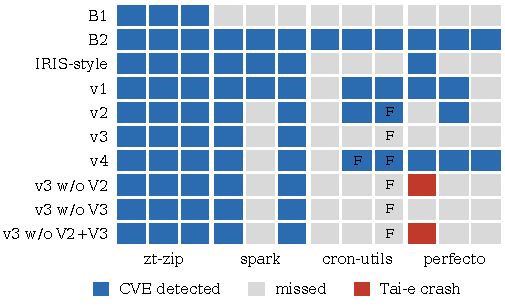
\includegraphics[width=\columnwidth]{figures/runs.pdf}
\caption{Buggy-version outcome of every run, three per subject (B1 and B2 are deterministic). F marks a run whose LLM driver failed V1 and fell back to the template. The bottom three rows are the v3 validator ablations.}
\Description{Grid with one row per configuration and three cells per subject. Blue cells are runs that detect the CVE, grey cells missed runs, red cells Tai-e crashes in V2-off ablations; an F marks fallback runs, for example two v4 runs on cron-utils.}
\label{fig:runs}
\end{figure}

We inspected every missed detection and every configuration's GT-relevant flows (Figure~\ref{fig:runs}), then categorised the sampled false positives.

\subsubsection{Missed detections}
Four causes explain the misses.

\nopagebreak[4]
\textbf{Missing entry setup (spark).} On the buggy version in run~1, the LLM drivers of v2 to v4 call 12 entries but never configure the static-file location, so the vulnerable handler is unreachable. In runs~0 and~2, they reach the resource lookup from the request path. The judge rejected these routes through library code, but the witness confirms that this sink is exploitable.

\textbf{Wrong overload and split state (perfecto-plugin).} Two v2 and v3 drivers pass null arguments to the plugin's setup method, so the compiler selects a deprecated Jenkins overload that the plugin does not override and the intended setup implementation remains unreachable. The third lists the setup method but never calls it. After v4's checks forced repairs, one driver still configured new objects and called the setup method on a separate object with no tainted state. These drivers compile successfully, but they either fail to call the intended setup implementation or call it on an object without the required tainted state. The v4 additions to V1 check for wrong overloads, missing declared-entry calls and calls on a different object from the one configured. These checks flag problems that compilation alone cannot detect and trigger repair requests.

\textbf{Driver fallback.} In total, \FallbackDrivers{} of the 48 generated drivers still fail V1 after repair, mostly by calling APIs that do not exist or making ambiguous overload calls. One ambiguous call came from a v4 entry-check repair. These runs use the template driver, including both v4 cron-utils detections and the fixed spark run with 1,528 alarms.

\textbf{Incorrect sink judgement (cron-utils).} N3 dismisses the Bean Validation message template as a harmless sink, and V3 accepts the verdict because its citations are valid. The verdict overlooks that message templates evaluate expression-language syntax, the cause of the CVE. The trusted-sink rule now stops such a verdict from overriding a trusted sink.

\subsubsection{False positives}
Three patterns explain the false alarms.

\textbf{Right method, wrong argument (zt-zip).} Many alarms reach the file constructor through its first argument, the trusted output directory, rather than its second, the archive entry name (Listing~\ref{lst:ztzip}). Patch-method metrics credit both, but only the second leads to the Zip Slip that the witness demonstrates.

\begin{figure}[t]
\centering
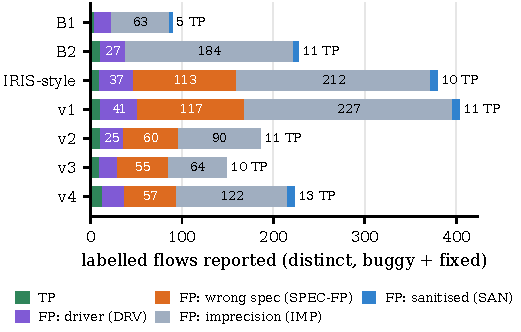
\includegraphics[width=\columnwidth]{figures/label_outcomes.pdf}
\caption{Judged flows reported by each configuration (distinct sampled flows over all subjects and versions), by LLM judgement and FP category.}
\Description{Horizontal stacked bars per configuration showing the number of judged flows that are true positives or false positives by category (driver, wrong specification, imprecision, sanitised). Imprecision dominates for every configuration; true positives are 5 to 13 per configuration.}
\label{fig:labels}
\end{figure}

\textbf{False-positive categories.} Of the \NumLabelled{} judged flows, \NumLabTP{} are TP and \NumLabFP{} FP (Figure~\ref{fig:labels}). In the unweighted sample, imprecision is the largest FP category (\PctLabIMP{}, \texttt{IMP}) as the shared helper methods connect unrelated callbacks or handlers that \texttt{1-call} analysis cannot separate. Wrong specifications (\PctLabSPEC{}, \texttt{SPEC-FP}) occur only with N2. Four in five mark exception messages containing paths as path-traversal sinks, which V2 accepts because they are well-typed. Driver modelling (\PctLabDRV{}, \texttt{DRV}) taints trusted output or configuration directories in both template and LLM drivers. Sanitised flows (\PctLabSAN{}, \texttt{SAN}) occur only on fixed versions, where the patch adds a check after the reported sink or runs the command as a build step. Triage removes nearly 30\% of the labelled imprecision flows (\VTwoLabIMP{} in v2 to \VThreeLabIMP{} in v3) but few specification errors (\VTwoLabSPEC{} to \VThreeLabSPEC{}).

\textbf{Changed security meaning (perfecto-plugin).} The patch moves command execution from the Jenkins controller into a build step. Data still reaches command execution, but under Jenkins' threat model this is intended behaviour. The witness confirms that the controller sink is gone; neither the automatic metrics nor triage captures this distinction.

To address RQ3, the misses come from missing sinks, incomplete LLM drivers and wrong triage verdicts. False alarms come mostly from imprecision, wrong inferred sinks and over-tainting drivers. These errors can remain after validation.

\subsection{Practical Feasibility (RQ4)}
\textbf{Resource use.} Successful Tai-e runs take seconds to about a minute, with Tai-e's sampled memory-peak field ranging from 355 to 3,263\,MB. The reported records contain \TotalCalls{} logical LLM calls, including the ablations omitted from Table~\ref{tab:cost}, many answered from a shared cache. The original runs sent 4,978 calls to the model, using 11.8M tokens and 4.83 hours of summed response time; cached replay times do not represent cold runs. IRIS-style has the largest triage load as it exhausts the 200-flow budget and leaves up to 1,622 spark flows unjudged per run.

\textbf{Stability.} Mean support for each API's most common N2 label is 93\% (counting absent or rejected labels as \texttt{none}), which measures consistency but not correctness. Mean pairwise Jaccard similarity of alarm sets ranges from 0.41 to 0.67 (Table~\ref{tab:cost}). Even v1, with its fixed template driver, reaches only 0.67 because N2's samples differ between runs while LLM drivers and triage add more variation. A single run can therefore miss a CVE that another finds (Figure~\ref{fig:runs}), so per-run detection rates matter alongside detection in any run. The deterministic baselines are reproducible: re-running B1 and B2 in a clean environment reproduced the alarm counts, detection flags and reported flow keys of all 16 runs.

\textbf{Practical limits.} The analysis ran on one laptop, with LLM inference provided by the shared endpoint. A full LLM pass took several hours, so we limited the study to four subjects, one model, three repetitions and 200 triage calls per run, and labelled a sample instead of all \NumFlows{} flows.

To address RQ4, the triage dominates LLM usage, and the triage limit leaves some alarms unreviewed. Variation across runs makes per-run detection rates necessary.

\section{Limitations}
\label{sec:limits}
\textbf{Detection evidence.} Patch-method overlap can credit unrelated or infeasible flows and miss relevant flows outside the patched methods. The witnesses confirm the four vulnerable sinks, but matching an alarm to such a sink does not validate its static route, and the other sampled alarms are checked only by the LLM judge.

\textbf{LLM-judged labels.} Due to time and resource constraints, all \NumLabelled{} labels come from one LLM judge so its errors may be anchored and correlated. Inclusion-probability weighting corrects the sampling imbalance but not wrong labels, so the precision estimates are provisional and have no quantified uncertainty. A flow key that recurs across runs may also stand for different driver assumptions.

\textbf{Development on the evaluated subjects.} The v4 rules address failures observed on the same four subjects, so their improvement is a development result, not evidence of transfer to unseen projects. Held-out subjects have yet to be tested.

\textbf{Use of a single LLM.} We evaluate four projects with one LLM and three repetitions per LLM configuration, so the findings cannot establish typical performance across projects, vulnerability classes or models. Public CVEs may have appeared in the model's training data and influenced its answers, but we cannot verify this. Fresh responses may also differ from the cached answers used for replay.

\textbf{Driver settings.} The template selects up to 300 entry methods, while N1 sees at most 60 candidates in its prompt. Fewer alarms may therefore partly reflect narrower entry coverage. Triage reviews at most 200 flows per run; the rest remain reported but unreviewed. Our IRIS-style configuration differs from published IRIS in its engine, model, subjects and how results are combined, so its results are not directly comparable.

\section{Conclusion}
The use of an LLM shifts the strengths and weaknesses of static taint analysis rather than uniformly improving it. Inferred specifications broaden coverage, generated drivers cut alarms but can omit essential entries, and triage can discard real vulnerabilities. A curated symbolic specification remains a strong baseline, reaching all four witness-validated sinks with about five times as many alarms as \tool{}. The targeted symbolic rules of \tool{} recover the detections that the initial pipeline lost and reach the same four sinks in at least one run per subject. To further improve the approach, we could check what inferred sinks mean, match driver budgets, vary the triage cap, evaluate unseen projects and have the labels reviewed independently.

\section*{AI Use Statement}
Claude Opus 5.5 assisted with literature review, code implementation, tests, flow labelling and report editing. GPT-5.6 Sol assisted with auditing and revising the paper's writing. I selected the baseline and subjects, designed the workflow, reviewed and debugged the implementation, ran the study and interpreted its failures. The analyzer uses SoCLaaS \texttt{qwen3.6:35b}. All in all, I am responsible for the submitted content.

\clearpage
\bibliographystyle{ACM-Reference-Format}
\bibliography{references}
\end{document}
